\documentclass{standalone}
\usepackage{tikz}
\usepackage{xcolor}
\usetikzlibrary{patterns, positioning}
\usetikzlibrary{shapes.misc}
\usepackage[outline]{contour}
\contourlength{1.5pt} 


\begin{document}
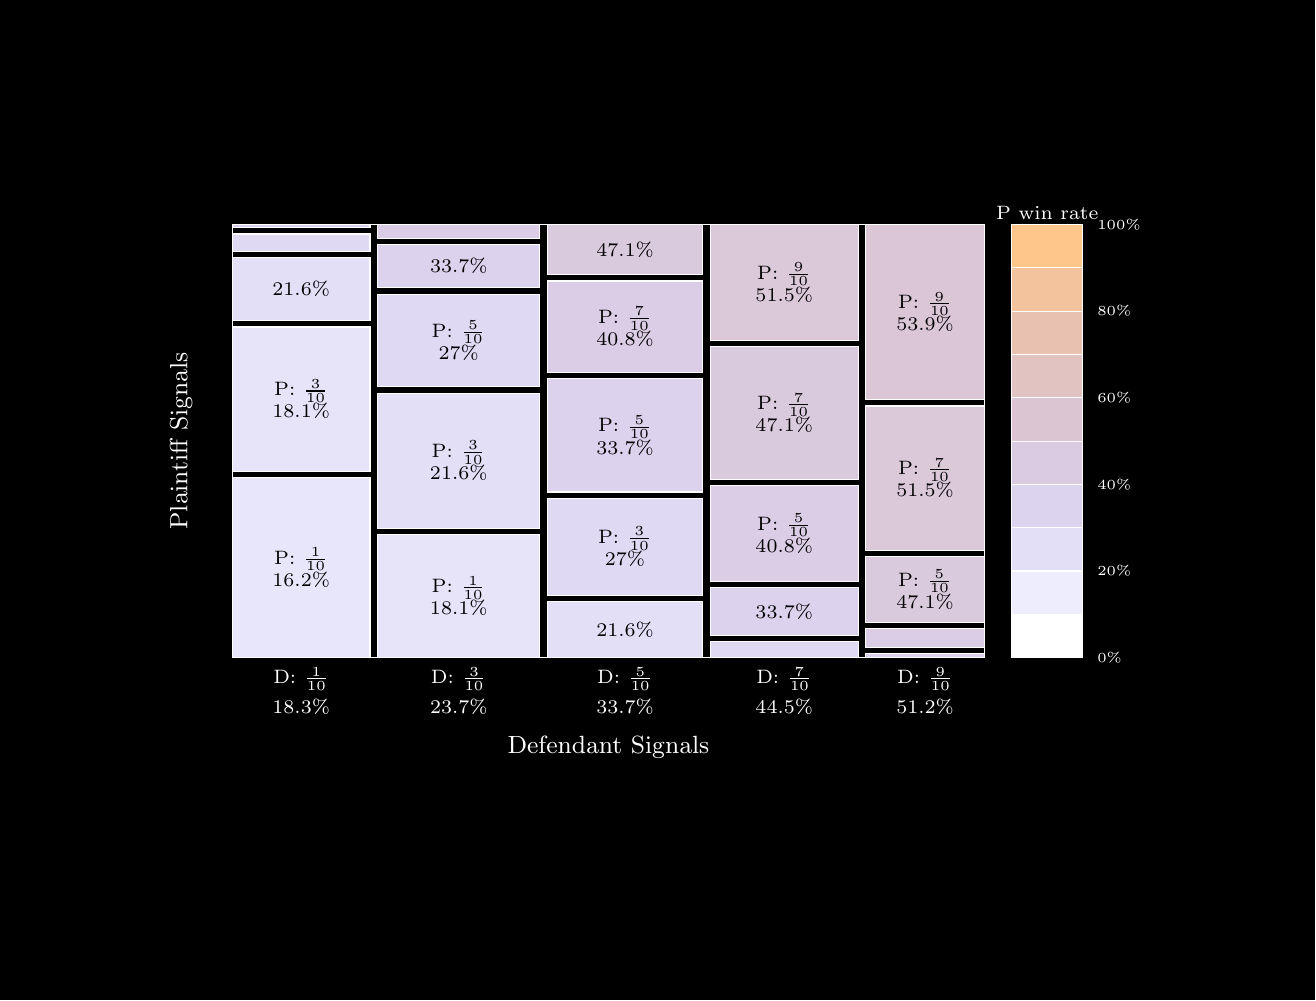
\begin{tikzpicture}
\newcommand{\DFractionOffset}{0.4}
\newcommand{\AxisLabelYAdjust}{-0.235}
\pagecolor{black}
\draw[fill=black, draw=none] (-2,-2) rectangle (14,10);
\draw[draw=white] (0.6,2) rectangle (10.15,7.5);
\draw[fill=blue!84!orange!16!white!66!white, draw=white] (0.6,2) rectangle (2.3476,4.2832);
\draw (1.4737984444213128, 3.141619361046671) node[font=\scriptsize, text=black, align=center] {P: $\frac{1}{10}$\\ 16.2\%};
\draw[fill=blue!82!orange!18!white!65!white, draw=white] (0.6,4.3632) rectangle (2.3476,6.1983);
\draw (1.4737984444213128, 5.280759563992288) node[font=\scriptsize, text=black, align=center] {P: $\frac{3}{10}$\\ 18.1\%};
\draw[fill=blue!78!orange!22!white!65!white, draw=white] (0.6,6.2783) rectangle (2.3476,7.081);
\draw (1.4737984444213128, 6.679624631302807) node[font=\scriptsize, text=black, align=center] {21.6\%};
\draw[fill=blue!73!orange!27!white!63!white, draw=white] (0.6,7.161) rectangle (2.3476,7.3797);
\draw[fill=blue!66!orange!34!white!62!white, draw=white] (0.6,7.4597) rectangle (2.3476,7.5);
\draw (1.4737984444213128, 1.6) node[anchor=north, font=\scriptsize, text=white] {18.3\%};
\draw (1.4737984444213128, {1.6 + \DFractionOffset}) node[anchor=north, font=\scriptsize, text=white] {D: $\frac{1}{10}$};
\draw[fill=blue!82!orange!18!white!65!white, draw=white] (2.4476,2) rectangle (4.5022,3.5608);
\draw (3.4749099264707066, 2.780412839134708) node[font=\scriptsize, text=black, align=center] {P: $\frac{1}{10}$\\ 18.1\%};
\draw[fill=blue!78!orange!22!white!65!white, draw=white] (2.4476,3.6408) rectangle (4.5022,5.3575);
\draw (3.4749099264707066, 4.499143725940918) node[font=\scriptsize, text=black, align=center] {P: $\frac{3}{10}$\\ 21.6\%};
\draw[fill=blue!73!orange!27!white!63!white, draw=white] (2.4476,5.4375) rectangle (4.5022,6.6163);
\draw (3.4749099264707066, 6.026887011988776) node[font=\scriptsize, text=black, align=center] {P: $\frac{5}{10}$\\ 27\%};
\draw[fill=blue!66!orange!34!white!62!white, draw=white] (2.4476,6.6963) rectangle (4.5022,7.2443);
\draw (3.4749099264707066, 6.970318142985212) node[font=\scriptsize, text=black, align=center] {33.7\%};
\draw[fill=blue!59!orange!41!white!60!white, draw=white] (2.4476,7.3243) rectangle (4.5022,7.5);
\draw (3.4749099264707066, 1.6) node[anchor=north, font=\scriptsize, text=white] {23.7\%};
\draw (3.4749099264707066, {1.6 + \DFractionOffset}) node[anchor=north, font=\scriptsize, text=white] {D: $\frac{3}{10}$};
\draw[fill=blue!78!orange!22!white!65!white, draw=white] (4.6022,2) rectangle (6.5712,2.7124);
\draw (5.586706919717463, 2.356221102274566) node[font=\scriptsize, text=black, align=center] {21.6\%};
\draw[fill=blue!73!orange!27!white!63!white, draw=white] (4.6022,2.7924) rectangle (6.5712,4.0226);
\draw (5.586706919717463, 3.407509853580082) node[font=\scriptsize, text=black, align=center] {P: $\frac{3}{10}$\\ 27\%};
\draw[fill=blue!66!orange!34!white!62!white, draw=white] (4.6022,4.1026) rectangle (6.5712,5.5408);
\draw (5.586706919717463, 4.821671323345051) node[font=\scriptsize, text=black, align=center] {P: $\frac{5}{10}$\\ 33.7\%};
\draw[fill=blue!59!orange!41!white!60!white, draw=white] (4.6022,5.6208) rectangle (6.5712,6.782);
\draw (5.586706919717463, 6.201403122382619) node[font=\scriptsize, text=black, align=center] {P: $\frac{7}{10}$\\ 40.8\%};
\draw[fill=blue!53!orange!47!white!58!white, draw=white] (4.6022,6.862) rectangle (6.5712,7.5);
\draw (5.586706919717463, 7.181020550343083) node[font=\scriptsize, text=black, align=center] {47.1\%};
\draw (5.586706919717463, 1.6) node[anchor=north, font=\scriptsize, text=white] {33.7\%};
\draw (5.586706919717463, {1.6 + \DFractionOffset}) node[anchor=north, font=\scriptsize, text=white] {D: $\frac{5}{10}$};
\draw[fill=blue!73!orange!27!white!63!white, draw=white] (6.6712,2) rectangle (8.5459,2.2039);
\draw[fill=blue!66!orange!34!white!62!white, draw=white] (6.6712,2.2839) rectangle (8.5459,2.8845);
\draw (7.608555167829337, 2.584240175065804) node[font=\scriptsize, text=black, align=center] {33.7\%};
\draw[fill=blue!59!orange!41!white!60!white, draw=white] (6.6712,2.9645) rectangle (8.5459,4.1842);
\draw (7.608555167829337, 3.5743650927422763) node[font=\scriptsize, text=black, align=center] {P: $\frac{5}{10}$\\ 40.8\%};
\draw[fill=blue!53!orange!47!white!58!white, draw=white] (6.6712,4.2642) rectangle (8.5459,5.9489);
\draw (7.608555167829337, 5.106524575217619) node[font=\scriptsize, text=black, align=center] {P: $\frac{7}{10}$\\ 47.1\%};
\draw[fill=blue!49!orange!51!white!57!white, draw=white] (6.6712,6.0289) rectangle (8.5459,7.5);
\draw (7.608555167829337, 6.764429212004328) node[font=\scriptsize, text=black, align=center] {P: $\frac{9}{10}$\\ 51.5\%};
\draw (7.608555167829337, 1.6) node[anchor=north, font=\scriptsize, text=white] {44.5\%};
\draw (7.608555167829337, {1.6 + \DFractionOffset}) node[anchor=north, font=\scriptsize, text=white] {D: $\frac{7}{10}$};
\draw[fill=blue!66!orange!34!white!62!white, draw=white] (8.6459,2) rectangle (10.15,2.0468);
\draw[fill=blue!59!orange!41!white!60!white, draw=white] (8.6459,2.1268) rectangle (10.15,2.3668);
\draw[fill=blue!53!orange!47!white!58!white, draw=white] (8.6459,2.4468) rectangle (10.15,3.2819);
\draw (9.397959730161267, 2.8643219375492186) node[font=\scriptsize, text=black, align=center] {P: $\frac{5}{10}$\\ 47.1\%};
\draw[fill=blue!49!orange!51!white!57!white, draw=white] (8.6459,3.3619) rectangle (10.15,5.1956);
\draw (9.397959730161267, 4.278729125401986) node[font=\scriptsize, text=black, align=center] {P: $\frac{7}{10}$\\ 51.5\%};
\draw[fill=blue!46!orange!54!white!57!white, draw=white] (8.6459,5.2756) rectangle (10.15,7.5);
\draw (9.397959730161267, 6.387782694629012) node[font=\scriptsize, text=black, align=center] {P: $\frac{9}{10}$\\ 53.9\%};
\draw (9.397959730161267, 1.6) node[anchor=north, font=\scriptsize, text=white] {51.2\%};
\draw (9.397959730161267, {1.6 + \DFractionOffset}) node[anchor=north, font=\scriptsize, text=white] {D: $\frac{9}{10}$};
\node[font=\small, text=white] at (5.375, {1.1 + \AxisLabelYAdjust}) {Defendant Signals};
\node[font=\small, text=white, rotate=90] at (-0.050000000000000044, 4.75) {Plaintiff Signals};
\draw[draw=white] (10.5,2) rectangle (11.4,7.5);
\draw (10.95, 7.65) node[font=\scriptsize, text=white] {P win rate};
\draw[fill=blue!100!orange!0!white!70!white, draw=white] (10.5,2) rectangle (11.4,2.55);
\draw[fill=blue!89!orange!11!white!67!white, draw=white] (10.5,2.55) rectangle (11.4,3.1);
\draw[fill=blue!78!orange!22!white!64!white, draw=white] (10.5,3.1) rectangle (11.4,3.65);
\draw[fill=blue!67!orange!33!white!62!white, draw=white] (10.5,3.65) rectangle (11.4,4.2);
\draw[fill=blue!56!orange!44!white!59!white, draw=white] (10.5,4.2) rectangle (11.4,4.75);
\draw[fill=blue!44!orange!56!white!56!white, draw=white] (10.5,4.75) rectangle (11.4,5.3);
\draw[fill=blue!33!orange!67!white!53!white, draw=white] (10.5,5.3) rectangle (11.4,5.85);
\draw[fill=blue!22!orange!78!white!51!white, draw=white] (10.5,5.85) rectangle (11.4,6.4);
\draw[fill=blue!11!orange!89!white!48!white, draw=white] (10.5,6.4) rectangle (11.4,6.95);
\draw[fill=blue!0!orange!100!white!45!white, draw=white] (10.5,6.95) rectangle (11.4,7.5);
\draw (11.46, 2) node[anchor=west, font=\tiny, text=white] {0\%};
\draw (11.46, 3.1) node[anchor=west, font=\tiny, text=white] {20\%};
\draw (11.46, 4.2) node[anchor=west, font=\tiny, text=white] {40\%};
\draw (11.46, 5.3) node[anchor=west, font=\tiny, text=white] {60\%};
\draw (11.46, 6.4) node[anchor=west, font=\tiny, text=white] {80\%};
\draw (11.46, 7.5) node[anchor=west, font=\tiny, text=white] {100\%};


\end{tikzpicture}
\end{document}